\section{Seller guide} \label{_venditore}
\subsection{Purpose of the section}
The goal of this section of the document is to describe what a seller can do using EmporioLambda.

\subsection{How access to the seller dashboard} \label{_adminlogin}
In order to access the seller dashboard, you have to sign in as seller. This can be done via these \hyperref[_signin]{istructions}.
Once you are signed in, you can access the seller dashboard by typing in the url "/admin/dashboard".
\begin{figure}[H]
    \centering
    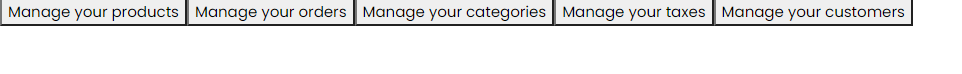
\includegraphics[width=\linewidth]{res/images/venditore/dashboard.png}
    \caption{Manage products}
\end{figure}

\subsection{How to access to different dashboards} \label{_dashboard}
In order to access to the dashboards that the service provides, you simply have to click on the button related to the dashboard. Then you will enter each different dashboard.

\subsubsection{Products dashboard} \label{_productmanagement}
\begin{figure}[H]
    \centering
    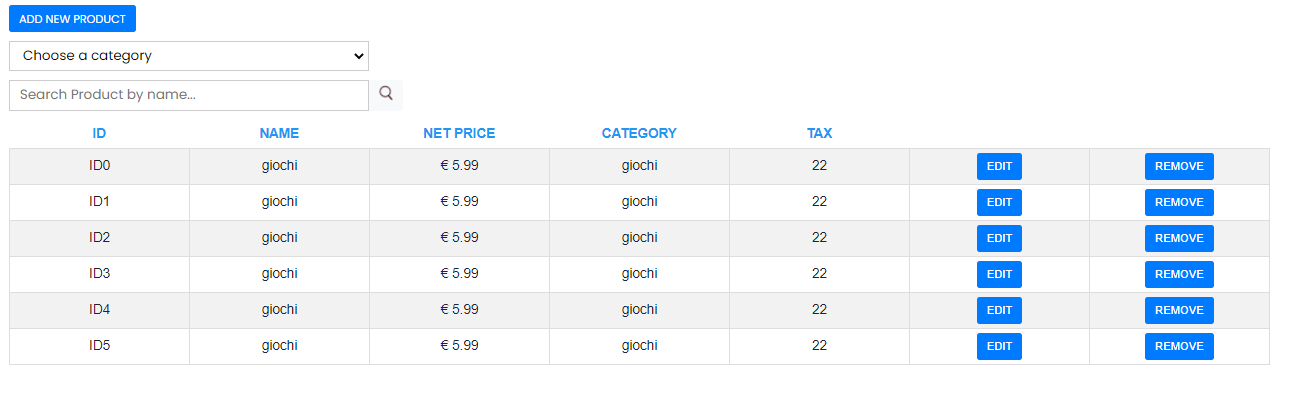
\includegraphics[width=\linewidth]{res/images/venditore/productmanagement.png}
    \caption{Products dashboard}
\end{figure}
\subsubsection{Orders dashboard} \label{_ordermanagement}
\begin{figure}[H]
    \centering
    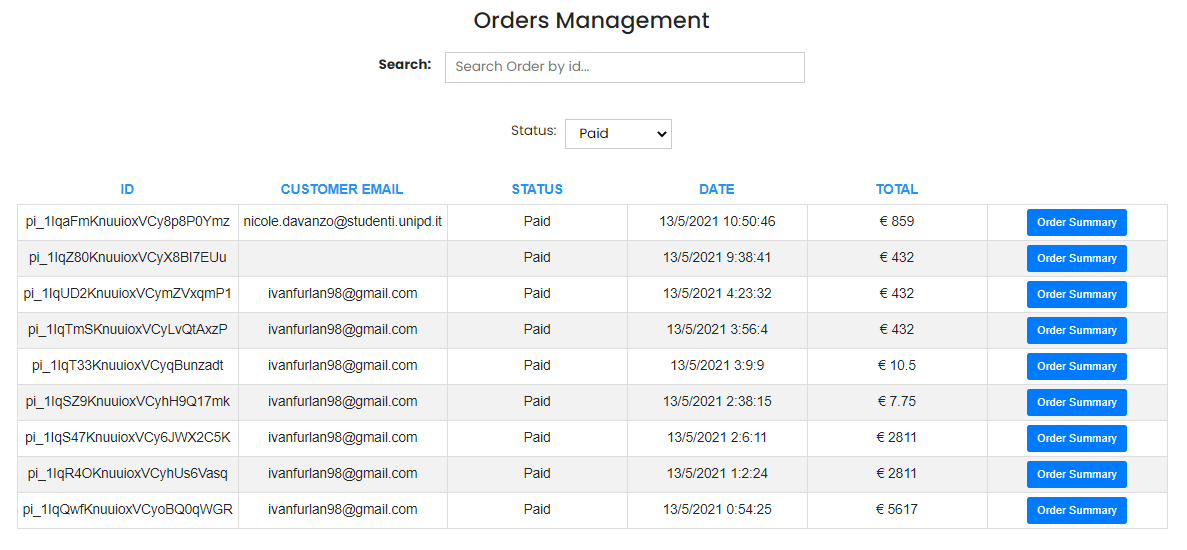
\includegraphics[width=\linewidth]{res/images/venditore/ordermanagement.png}
    \caption{Orders dashboard}
\end{figure}
\subsubsection{Categories dashboard} \label{_categorymanagement}
\begin{figure}[H]
    \centering
    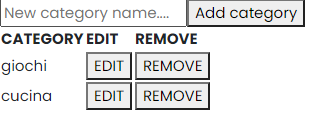
\includegraphics[width=\linewidth]{res/images/venditore/categorymanagement.png}
    \caption{Categories dashboard}
\end{figure}
\subsubsection{Tax dashboard} \label{_taxmanagement}
\begin{figure}[H]
    \centering
    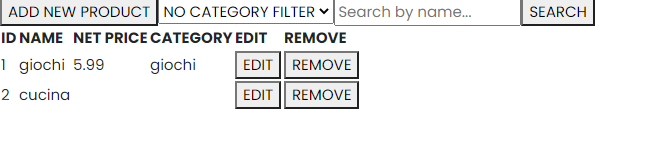
\includegraphics[width=\linewidth]{res/images/venditore/taxmanagement.png}
    \caption{Tax dashboard}
\end{figure}
\subsubsection{Customers dashboard} \label{_customermanagement}
\begin{figure}[H]
    \centering
    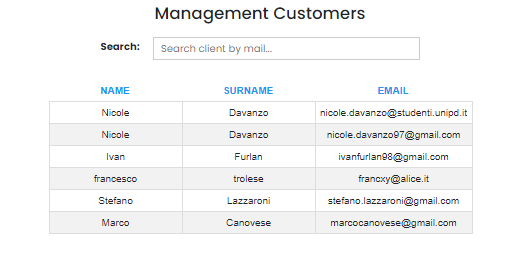
\includegraphics[width=\linewidth]{res/images/venditore/customermanagement.png}
    \caption{Customers dashboard}
\end{figure}


\subsection{How to add a product}\label{_addProduct}
In order to add a product, you have to click on the "Add new product" button in the \hyperref[_productmanagement]{Product Dashboard}.
Here you have to fill each field with the correct data. Then press the "Save" button that adds the product to the e-commerce platform.
\begin{figure}[H]
    \centering
    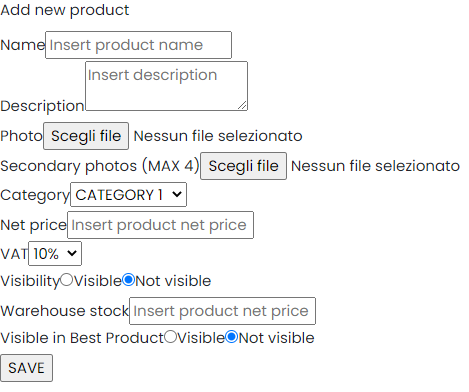
\includegraphics[width=30em]{res/images/venditore/addproduct.png}
    \caption{Add product}
\end{figure}

\subsection{How to find a product}\label{_findProduct}
There are three ways to find a product:
\begin{itemize} 
    \item \textbf{Selecting a category};
    \item \textbf{Searching the name with the search bar}. 
    \item \textbf{Using both};
\end{itemize}

\begin{figure}[H]
    \centering
    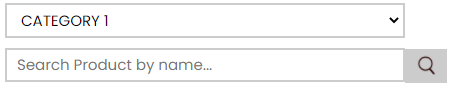
\includegraphics[width=20em]{res/images/venditore/categoryandsearchbar.png}
    \caption{Category Dropdown - Search bar}
\end{figure}

\subsection{How to edit a product}\label{_editProduct}
In order to edit a product, select the desired product from the product list. If you prefer you can also filter the list by category or by name. Then click "edit".
Here you have to fill each field with the correct data. Then press the "Save" button that saves the changes of the selected product.
\begin{figure}[H]
    \centering
    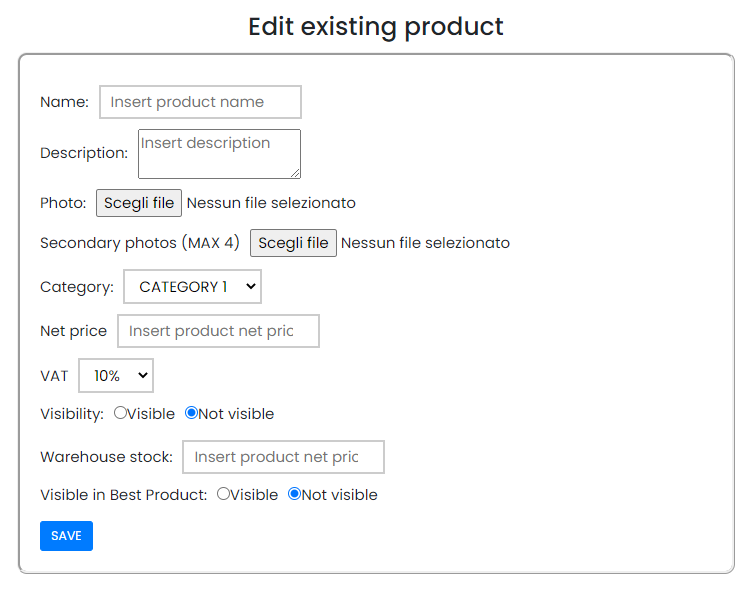
\includegraphics[width=30em]{res/images/venditore/editproduct.png}
    \caption{Edit product}
\end{figure}

\subsection{How to remove a product}\label{_removeProduct}
In order to delete a product, select the desired product from the product list. If you prefer you can also filter the list by category or by name. Then click "remove".

\subsection{How to find an order}\label{_findOrder}
In order to find an order, you have to type the ID in the search bar.
\begin{figure}[H]
    \centering
    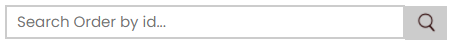
\includegraphics[width=20em]{res/images/venditore/ordersearchbar.png}
    \caption{Order search bar}
\end{figure}
Then will be displayed the order that has the desired ID. If there are no orders with the searched id, the table will be empty.

\subsection{How to get an order summary}\label{_orderSummary}
In order to find an order, from the \hyperref[_ordermanagement]{Orders dashboard}, you have to simply click the Order Summary button. If you prefer, you can search a product.
\begin{figure}[H]
    \centering
    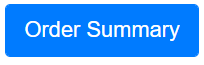
\includegraphics[width=10em]{res/images/venditore/ordersummarybutton.png}
    \caption{Order Summary Button}
\end{figure}

\subsection{How to add a category}\label{_addCategory}
In order to add a category, from the \hyperref[_categorymanagement]{Category dashboard}, you have to simply click the Add New Category button.
A small popover will appear.
\begin{figure}[H]
    \centering
    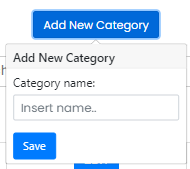
\includegraphics[width=15em]{res/images/venditore/addcategory.png}
    \caption{Add New Category Popover}
\end{figure}

\subsection{How to find a category}\label{_findCategory}
In order to find a category, from the \hyperref[_categorymanagement]{Category dashboard}, you have to simply type the category name.
\begin{figure}[H]
    \centering
    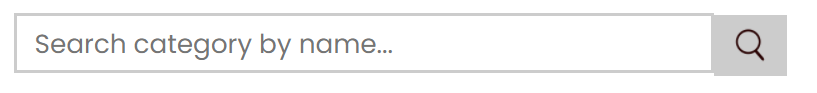
\includegraphics[width=15em]{res/images/venditore/categorysearchbar.png}
    \caption{Category search bar}
\end{figure}

\subsection{How to edit a category}\label{_editCategory}
In order to edit a category, from the \hyperref[_categorymanagement]{Category dashboard}, you have to simply click the EDIT button.
A small popover will appear.
You can always search the desired category using the \hyperref[_findCategory]{searchbar}.
\begin{figure}[H]   
    \centering
    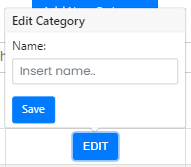
\includegraphics[width=15em]{res/images/venditore/editcategory.png}
    \caption{Edit Category Popover}
\end{figure}

\subsection{How to remove a category}\label{_removeCategory}
In order to delete a category, from the \hyperref[_categorymanagement]{Category dashboard}, you have to simply click the X button.
You can always search the desired category using the \hyperref[_findCategory]{searchbar}.

\subsection{How to add a tax}\label{_addTax}
In order to add a tax to the tax list you have to click on the button "Add new tax". A small popover will appear and you will be able to set the description and the amount of the tax.
\begin{figure}[H]
    \centering
    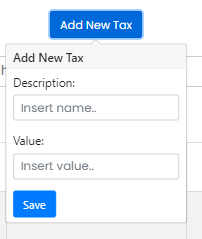
\includegraphics[width=15em]{res/images/venditore/addtax.png}
    \caption{Add New Tax Popover}
\end{figure}
After you click on "Save" the tax will now be available to use on the products.

\subsection{How to find a tax}\label{_findTax}
In order to find a tax, you have to simply type the category name in the Search box.
\begin{figure}[H]
    \centering
    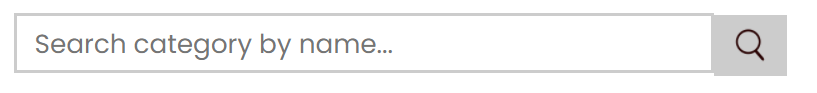
\includegraphics[width=15em]{res/images/venditore/categorysearchbar.png}
    \caption{Category search bar}
\end{figure}

\subsection{How to edit a tax}\label{_editTax}
In order to edit a tax, you have to simply click the EDIT button.
A small popover will appear where you can change the amount and the description of that particular tax.
\begin{figure}[H]    
    \centering
    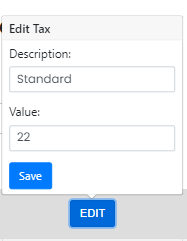
\includegraphics[width=15em]{res/images/venditore/edittax.png}
    \caption{Edit Tax Popover}
\end{figure}

\subsection{How to remove a tax}\label{_removeTax}
In order to delete a tax, select the desired product from the tax list. If you prefer you can also filter the list by tax name. Then click the X button.

\subsection{How to find a customer}\label{_findCustomer}
In order to find a customer inside the web app you can search directly inside the list on the main page or you can click on "Search client by email.." and write the specific email of the customer you are searching. \hyperref[_categorymanagement]{Category dashboard}, you have to simply type the category name.
\begin{figure}[H]
    \centering
    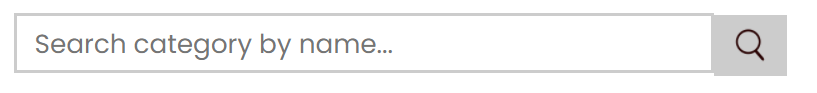
\includegraphics[width=15em]{res/images/venditore/categorysearchbar.png}
    \caption{Category search bar}
\end{figure}

\subsection{How to contact a customer}\label{_contactCustomer}
In order to contact a costumer, select the right one in the list and click on the email. The website will redirect you inside the default application you user to send email with the "To:" field already set up.

\subsection{How to manage your credentials and personal informations} \label{_credentials}
In order to be able to manage your credentials you have to be signed in. This action can be done via these \hyperref[_signin]{instructions}.
Then you have to access the profile page by clicking the profile button.
\begin{figure}[H]
    \centering
    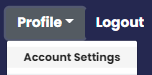
\includegraphics[width=10em]{res/images/cliente/profileaccount.png}
    \caption{Profile Button}
\end{figure}

Here you can edit your current password and your current e-mail.
To edit the password:
\begin{itemize} 
    \item \textbf{Old password}: insert the old password;
    \item \textbf{New password}: insert the new password; 
    \item \textbf{Confirm new password}: re-insert the new password. This step ensures the user not to  mistype the password.
\end{itemize}

\begin{figure}[H]
    \centering
    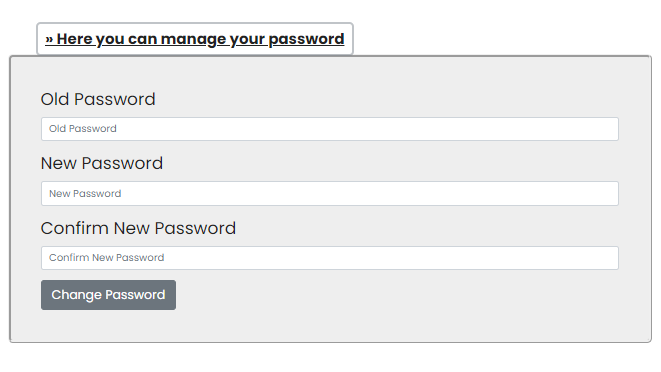
\includegraphics[width=30em]{res/images/cliente/credentialpwd.png}
    \caption{Change password form}
\end{figure}

To edit the e-mail:
\begin{itemize} 
    \item \textbf{New password}: insert the new e-mail; 
    \item \textbf{Confirm new password}: re-insert the new e-mail. This step ensures the user not to  mistype the e-mail.
\end{itemize}

\begin{figure}[H]
    \centering
    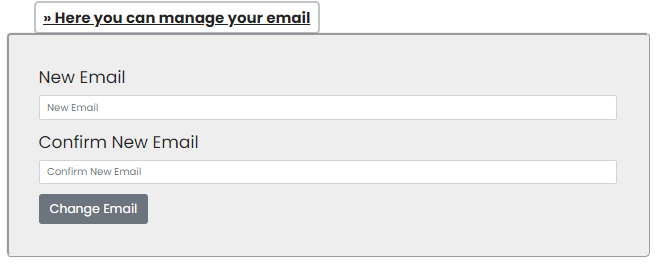
\includegraphics[width=30em]{res/images/cliente/credentialemail.png}
    \caption{Change email form}
\end{figure}

To edit your personal informations:
\begin{itemize} 
    \item \textbf{New Name}: insert the new name; 
    \item \textbf{New Surname}:insert the new surname.
\end{itemize}

\begin{figure}[H]
    \centering
    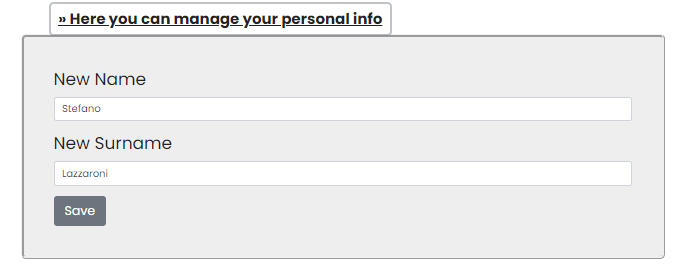
\includegraphics[width=30em]{res/images/cliente/personalinfo.png}
    \caption{Change personal informations form}
\end{figure}

\subsection{How to delete your account} \label{_delete}
In order to be able to request an account deletion you have to be signed in. This action can be done via these \hyperref[_signin]{instructions}.
Then you have to access the profile page by clicking the profile button.
When you click the "Request account deletion" button, you will be delete from site.
\begin{figure}[H]
    \centering
    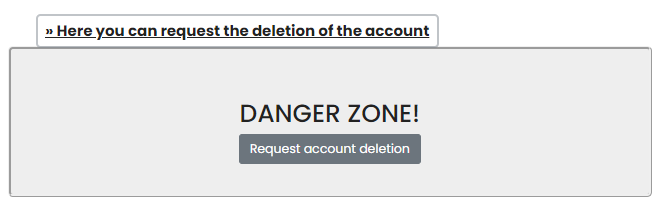
\includegraphics[width=30em]{res/images/cliente/delete.png}
    \caption{Delete Account Request}
\end{figure}

\subsection{How to manage your device} \label{_device}
In order to be able to request an account deletion you have to be signed in. This action can be done via these \hyperref[_signin]{instructions}.
Then you have to access the profile page by clicking the profile button.
Here you can:
\begin{itemize} 
    \item \textbf{Forget a device}: you have to click on the "Delete" button next to the selected device; 
    \item \textbf{Forget all devices}:click on the "Froget all devices" button;
    \item \textbf{logout from all devices}:click on the "Logout from all devices" button.
\end{itemize}

\begin{figure}[H]
    \centering
    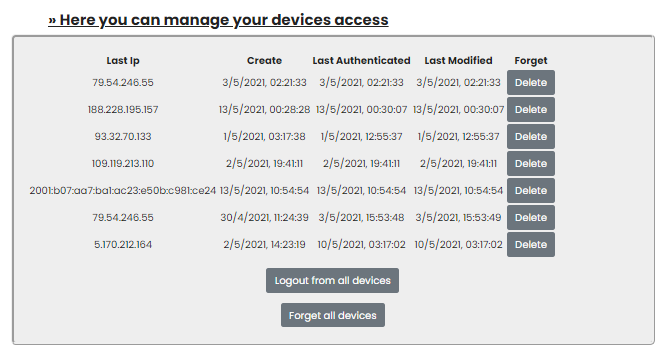
\includegraphics[width=30em]{res/images/cliente/device.png}
    \caption{Device Management}
\end{figure}

